\section{Seismic}

\section{Thermal}

We derive the thermal noise of a system using the fluctuation-dissipation
theorem which describes a relationship between the fluctuation of a system
and its dissipation. The starting point for our thermal noise calculations
is the Callen form of the theorem. \cite{Saulson,Callen}

The \ac{psd} of the thermal noise is defined,
\begin{align}
S_{xx}(\omega) =& \frac{4 k_B T}{\omega^2} \Re (Y(\omega)) \\
    =& \frac{4 k_B T}{\omega^2} \Re (Y(\omega))
\end{align}
For a system with velocity damping($b$), $F_{\mathrm{ext}} = m\ddot{x} + b\dot{x} + kx$,
we can rewrite the \ac{psd} as,
\begin{align}
S_{xx}(\omega) =& \frac{4 k_B T}{\omega^2} \Re (Y(\omega)) \\
    =& \frac{4 k_B T b / \omega^2}{ b^2 + (m \omega - k/\omega)^2}
\end{align}
Notice that as the damping coefficient goes to zero, this function becomes a
delta function at the resonant frequency, $\omega_0 = \sqrt{k/m}$.

That works for something like gas damping. However, we are more interested in
the thermal noise due to internal damping where the damping is essentially
absorbed into the spring coefficient making it complex. This changes the
dependence of the \ac{psd} on $\omega$. Taking this new form of damping,
$F_{\mathrm{ext}} = m\ddot{x} + k(1+i\phi)x$, where $\phi$ is called the
loss angle (for small values of $\phi$) we can write the PSD as,
\begin{align}
S_{xx}(\omega) = & \frac{4 k_B T k \phi / \omega}{(k \phi)^2 +
    (m \omega^2 - k)^2}
\end{align}
In this case we still have the peak at the resonant frequency, however the form
of the noise is different above and below the resonant frequency.

Now we will derive the thermal noise for our small mirror assembly. We are
concerned with thermal noise due to the epoxy used to glue the fibers to the
mass. We start with the Lagrangian to get the dynamics of the system and
compute the admittance.
\begin{align}
\begin{split} \label{eq:fullT}
T &= \frac{1}{2} M \dot{x}^2 +
    \frac{1}{2}I_M \left( \dot{\eta_1}^2 + \dot{\eta_2}^2 \right) \\
    &\quad + \frac{1}{2} m \left(
    \dot{x} + r_M \dot{\eta_1}
    + r_{\mathrm{cm}} \dot{\theta_1} \right)^2 \\
    &\quad + \frac{1}{4} m \left(
    2 \dot{x} - r_M \left(
    \dot{\eta_1}
    + \sqrt{3} \dot{\eta_2} \right)
    + 2r_{\mathrm{cm}} \dot{\theta_2} \right)^2 \\
    &\quad + \frac{1}{4} m \left(
    2 \dot{x} - r_M \left(
    \dot{\eta_1}
    - \sqrt{3} \dot{\eta_2} \right)
    + 2r_{\mathrm{cm}} \dot{\theta_3} \right)^2 \\
    &\quad + \frac{1}{2} I_m \left[
    \left( \dot{\theta_1} + \dot{\eta_1} \right)^2
    + \frac{1}{2} \left( 2\dot{\theta_2} - \dot{\eta_1} - \sqrt{3} \dot{\eta_2} \right)^2
    + \frac{1}{2} \left( 2\dot{\theta_3} - \dot{\eta_1} + \sqrt{3} \dot{\eta_2} \right)^2
    \right]
\end{split} \\
\label{eq:fullV}
V &= \frac{E l_y l_x^3}{8t} \left( \theta_1^2 + \theta_2^2 + \theta_3^2 \right)
\end{align}
Where $x$ is the position of the mirror, $\eta_1$ and $\eta_2$ are the pitch and yaw
of the mirror, and $\theta_i$ are the angles of each fiber attachment nub with
respect to the mirror.

The equations of motion become quite complex, so we simplify the system by only
looking at the contribution from the longitudinal mode. The effects of the pitch
and yaw modes should not contribute at first order for a perfectly aligned
system, so we can simplify \eqref{eq:fullT} and \eqref{eq:fullV} with,
\begin{align}
T &= \frac{1}{2} M\dot{x}^2
    + \frac{3}{2} m\left(\dot{x}+r_{\mathrm{cm}}\dot{\theta} \right)^2
    + \frac{3}{2} I\dot{\theta}^2 \\
V &= \frac{E l_y l_x^3}{8t}\theta^2 
\end{align}
making some substitutions,
\begin{align}
m_t &= M+3m \, , \\
I_t &= 3 \left( mr_{\mathrm{cm}}^2+I \right) \, , \\
K &= \frac{E l_y l_x^3}{4t} \, ,
\end{align}
the Lagrangian becomes,
\begin{align}
\frac{1}{2} \left( m_t \dot{x}^2 +6mr_{\mathrm{cm}}\dot{x}\dot{\theta}
+ I_t\dot{\theta}^2 -K\theta^2 \right) \, .
\end{align}
We can then find the equations of motion with an external force in
the $x$ direction,
\begin{align}
F_{\mathrm{ext}} &= \frac{d}{dt}\frac{\partial L}{\partial \dot{x}}
  - \frac{\partial L}{\partial x} \,.
\end{align}
The two equations of motion become,
\begin{align}
F_{\mathrm{ext}} &= m_t \ddot{x} + 3mr_{\mathrm{cm}}\ddot{\theta} \\
0 &= 3mr_{\mathrm{cm}}\ddot{x} + I_t\ddot{\theta} + K\theta \, .
\end{align}
We can then solve for the impedence in the frequency domain,
\begin{align}
Z = \frac{F_{\mathrm{ext}}}{i\omega x} &= m_t i\omega
  + 3mr_{\mathrm{cm}}i\omega \frac{\theta}{x} \,,
\end{align}
where, from the second equation,
\begin{align}
\frac{\theta}{x} &= \frac{3mr_{\mathrm{cm}}\omega^2}{K-I_t\omega^2} \,.
\end{align}
We need the real part of the admittance, $Y=1/Z$.
\begin{align}
Y &= \frac{iI_t\omega^2-iK}{\omega m_t(K-I_t\omega^2) + (3mr_{\mathrm{cm}})^2\omega^3}
\end{align}
The real part of $Y$ is then,
\begin{equation}
\frac{K_0 \phi \omega (3mr_{\mathrm{cm}})^2}{ \left(
  m_tK_0 + \omega^2 \left( (3mr_{\mathrm{cm}})^2 -m_tI_t \right) \right)^2
  + (m_tK_0 \phi)^2 }
\end{equation}
And the thermal noise in the $x$ direction is (we have taken $\phi$ to be small),
\begin{equation}
S_{xx}(\omega) = \frac{4k_BT}{\omega} \left[
  \frac{K_0\phi (3mr_{\mathrm{cm}})^2}{\left( m_tK_0 + \omega^2 \left( (3mr_{\mathrm{cm}})^2 -m_tI_t \right)
  \right)^2 }
  \right] \label{eq:tnoisesusfull}
\end{equation}

When $\omega$ is below the resonant frequency,
\begin{align}
S_{xx}(\omega) &= \frac{4k_BT}{m_t^2 \omega}
  \frac{\phi(3mr_{\mathrm{cm}})^2}{K_0} \label{eq:generalmassgluenoise} \\
S_{xx}(\omega) &= \frac{16k_BT\phi t(3mr_{\mathrm{cm}})^2}{m_t^2 \omega El_yl_x^3}
\end{align}
It is desirable to make the nubs much smaller than the mirror.
So, we can simplify the equation to,
\begin{align}
S_{xx}(\omega) &= \frac{36k_BT\phi t l_yl_z^4\rho^2}{M^2\omega El_x} \,.
\end{align}
Now, it is obvious that we want to make the nubs so that the center of mass is
close to the mirror, the thickness of the glue is small, and the glue area is
large in the dimension along the axis of the mirror.

For our situation we have actually arrived at a cone shaped nub which provides
for a large base and a short $r_{\mathrm{cm}}$. Going back to eq.
\eqref{eq:generalmassgluenoise} we make the approximations to get
\begin{align}
S_{xx}(\omega) &= \frac{4k_BT\phi(3mr_{\mathrm{cm}})^2}{M^2 \omega K_0}
\end{align}
The mass of a cone is $\frac{1}{3} \pi R^2 l_z \rho$, $r_{\mathrm{cm}}$ is
$\frac{1}{4} l_z$, and $K_0 = \frac{3\pi ER^4}{4t}$.
\begin{align}
S_{xx}(\omega) &= \frac{k_BT\phi \pi t l_z^4\rho^2}{3M^2 \omega E}
\end{align}
The noise is independent of the radius of the base of the cone, but depends
heavily on the length of the cone. The expressions for $K_0$ assume that
$t$ is large compared to $\frac{R^2}{2R_m}$. Figure \ref{fig:tnoisec}
depicts the \ac{asd} of this epoxy thermal noise contribution to the cavity
length noise.

\begin{figure}[htbp]
  \tikzsetnextfilename{tnoisecone}
  \begin{tikzpicture}
  \begin{loglogaxis}[
    xlabel={Frequency $\left( Hz \right)$},
    ylabel={Thermal Noise $\left( m/\sqrt{H\!z} \right)$},
    grid=minor,
  ]
  \addplot[red] table {python/tnoisecone.dat};
  \end{loglogaxis}
  \end{tikzpicture}
  \caption[Epoxy Thermal Noise Contribution to Trap Length]{This is a plot
    of the thermal noise from the epoxy used to glue the small conical nubs
    for the fiber suspension. This includes the resonance which comes from
    the full expression in \eqref{eq:tnoisesusfull}.}
  \label{fig:tnoisec}
\end{figure}

%\begin{figure}[htbp]
%	\centering
%		\includegraphics{./figures/tnoisecone.eps}
%	\caption[Thermal Noise From Epoxy in Small Mirror Suspension]{Noise contribution
%        from epoxy thermal noise.}
%	\label{fig:tnoisecone}
%\end{figure}

\section{Laser Frequency}

Laser frequency noise couples into the measurement significantly due to the
interferometric nature of the experiment.
The coupling goes as the length of the cavity as discussed in section
\ref{sec:lin_short}.

\section{Laser Intensity}

As mentioned in chapter \ref{ch:psl} the laser has an intensity noise
specification of \ac{rin} -150 $dB/Hz$. This is equivalent to a noise
spectrum of $10^{-7.5} W/\sqrt{H\!z}$ for a $1 W$ beam.
Measurements of the intensity noise in the lab, however, differ from this
value in the frequency range we are interested in.
The measured intensity noise compared to the laser specification is shown
in figure \ref{fig:intensitynoise}.

\begin{figure}[htbp]
  \tikzsetnextfilename{intensitynoise}
  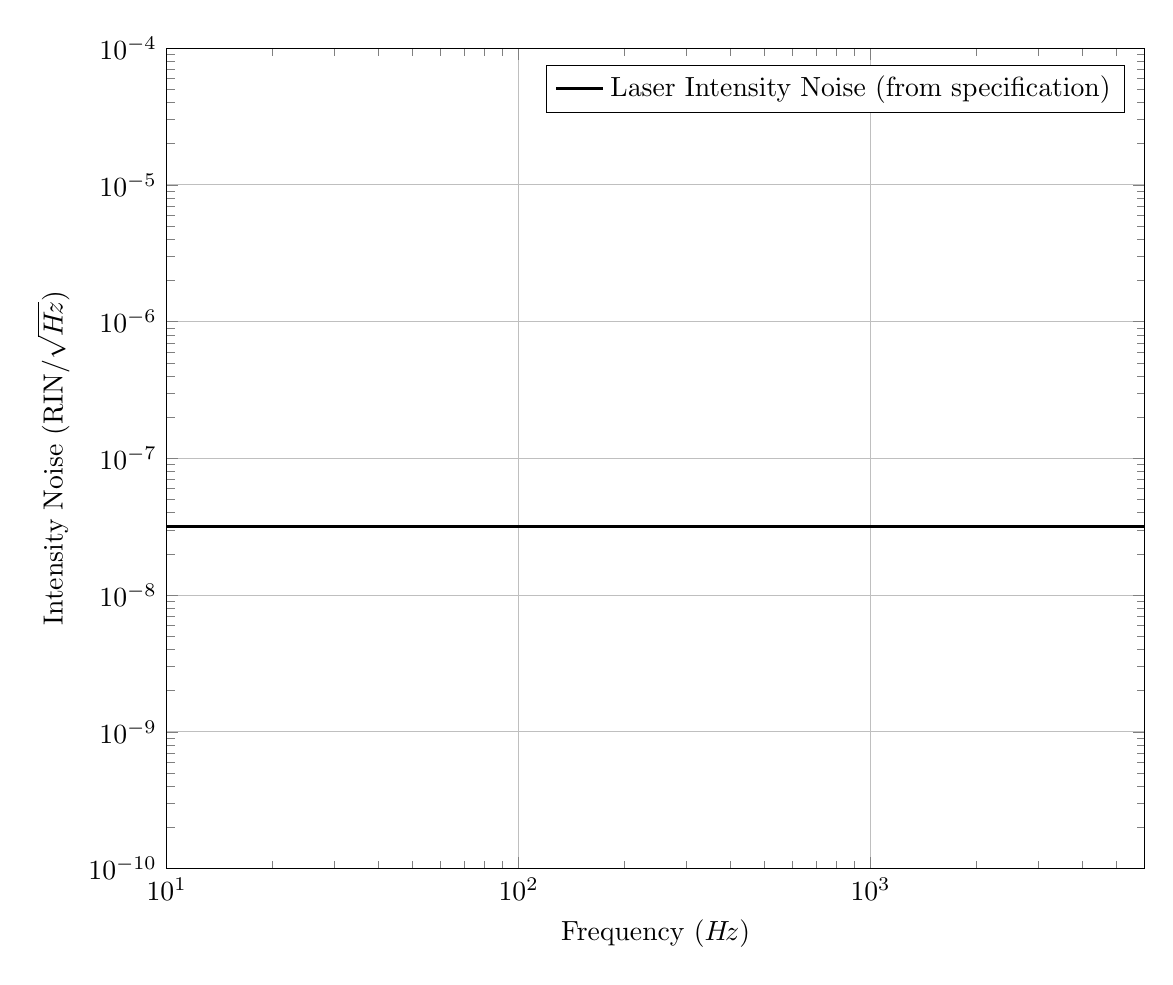
\begin{tikzpicture}
  \begin{loglogaxis}[
    height=12cm,
    width=14cm,
    xlabel={Frequency $(H\!z)$},
    ylabel={Intensity Noise $(\mathrm{RIN}/\sqrt{H\!z})$},
    xmin=10,
    xmax=6000,
    ymin=1e-10,
    ymax=1e-4,
    grid=major,
    legend cell align=left,
  ]
  \addplot[black,domain=10:6000,very thick] {10^(-7.5)};
  \addlegendentry{Laser Intensity Noise (from specification)}
  \end{loglogaxis}
  \end{tikzpicture}
  \caption[Intensity Noise]{This is the laser intensity noise}
  \label{fig:intensitynoise}
\end{figure}


\section{Electronics}



\section{Noise Budget}

\begin{figure}[htbp]
  \tikzsetnextfilename{noisebudgetjune}
  \begin{tikzpicture}
  \begin{loglogaxis}[
    height=12cm,
    width=14cm,
    xlabel={Frequency $(H\!z)$},
    ylabel={Trap Length Noise $(m/\sqrt{H\!z})$},
    xmin=10,
    xmax=6000,
    ymin=1e-16,
    ymax=1e-8,
    grid=major,
    legend cell align=left,
  ]
  \addplot[blue,very thick] table[x index=0,y index=1]
    {./matlab_traces/june_noises.dat};
  \addlegendentry{Measured Trap Length Noise}
  \addplot[green,very thick] table[x index=0,y index=2]
    {./matlab_traces/june_noises.dat};
  \addlegendentry{Laser Frequency Noise}
  \addplot[black,very thick] table[x index=0,y index=3]
    {./matlab_traces/june_noises.dat};
  \addlegendentry{Laser Intensity Noise}
  \addplot[red,very thick] table[x index=0,y index=4]
    {./matlab_traces/june_noises.dat};
  \addlegendentry{Seismic Noise}
  \addplot[purple,very thick,domain=10:10000] {2.3e-9/x/x};
  \end{loglogaxis}
  \end{tikzpicture}
  \caption[Noise Budget]{This is the noise budget which includes the measured
    cavity length noise with a stable optical spring.}
  \label{fig:noisebudget}
\end{figure}

\begin{figure}[htbp]
	\centering
		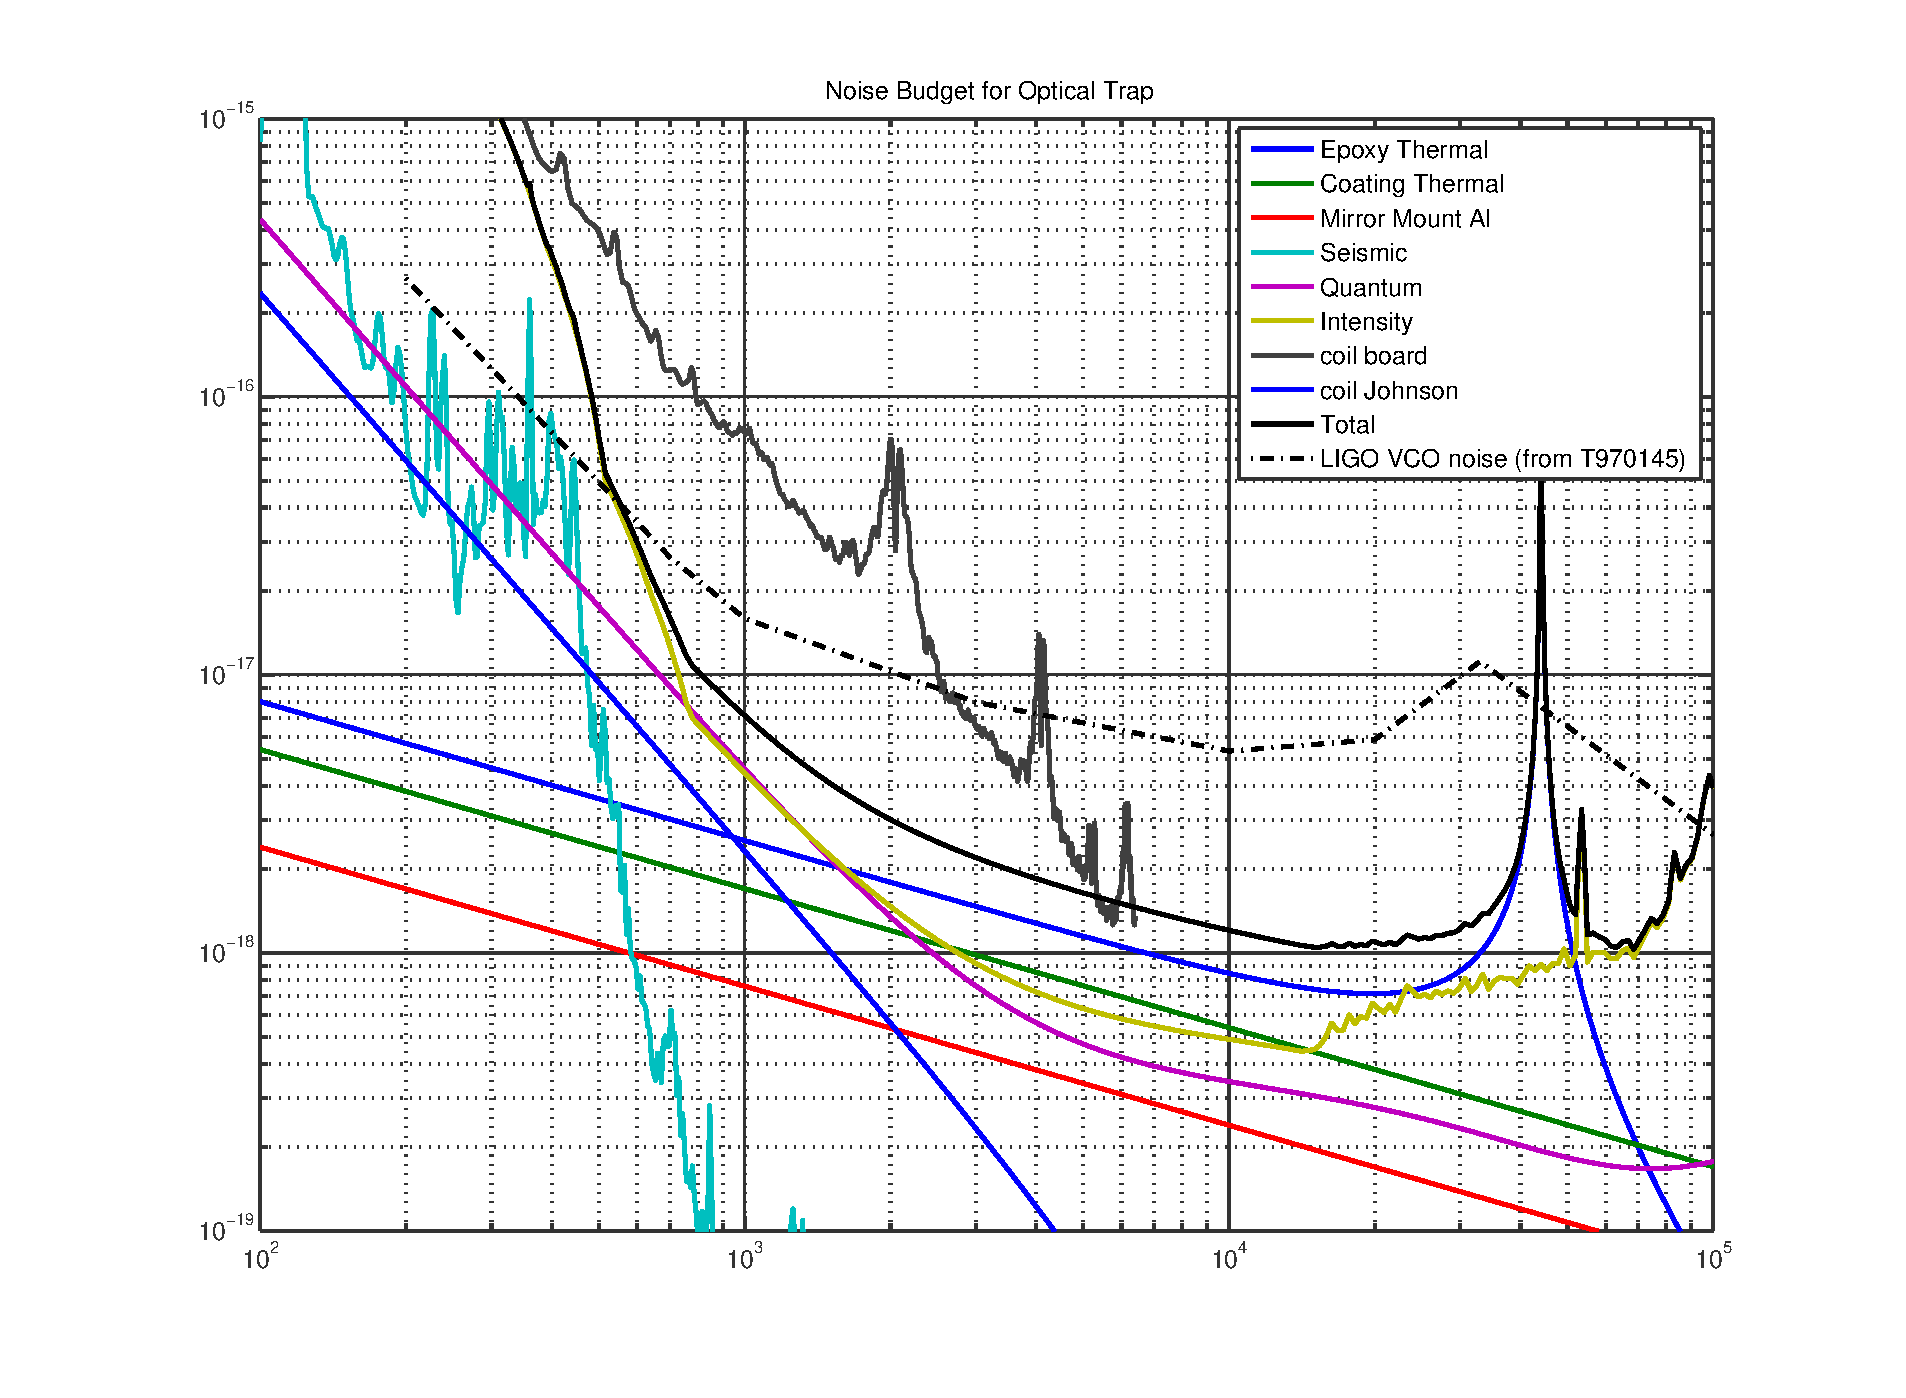
\includegraphics[width=15cm]{./figures/noise_budget.eps}
	\caption[Noise Budget]{Noise budget}
	\label{fig:noise_bud}
\end{figure}

\begin{figure}[htbp]
	\centering
		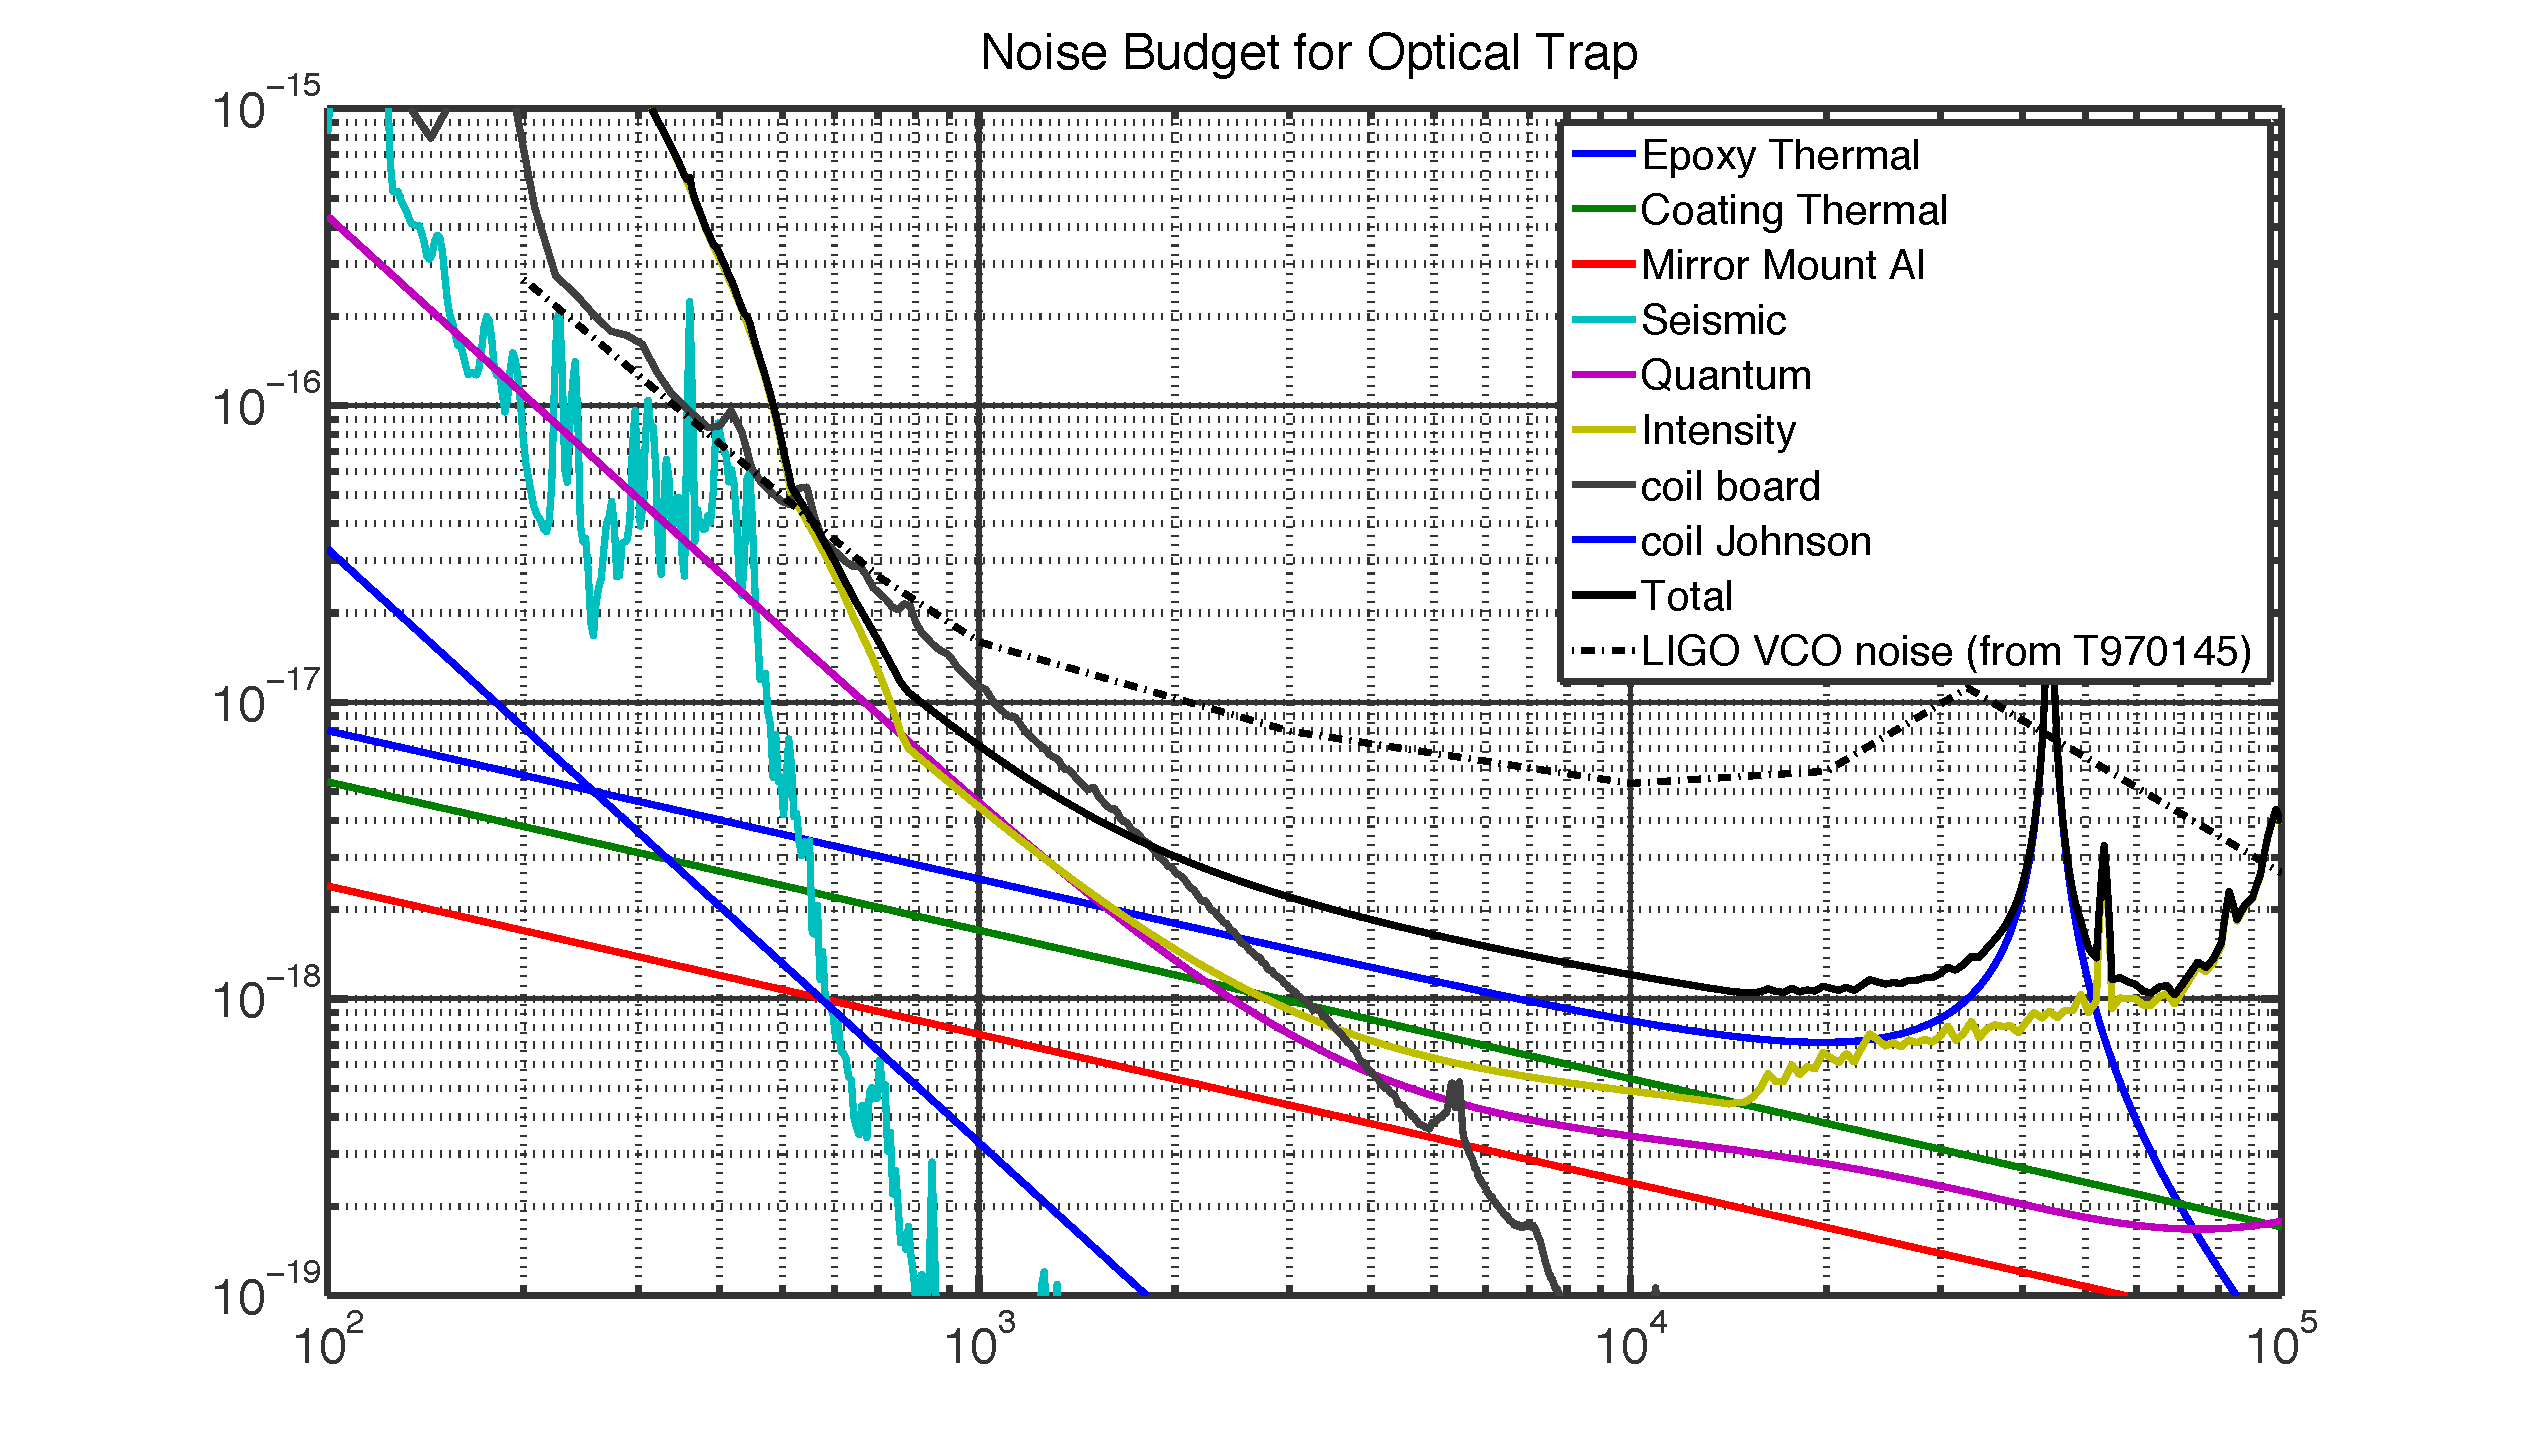
\includegraphics[width=15cm]{./figures/NoiseBudgetBoard.pdf}
	\caption[Noise Budget Board]{Noise budget with coil driver board noise}
	\label{fig:noise_bud_brd}
\end{figure}

\section{Vacuum Requirements for Optical Trap}

It is desired to have an understanding of limits of vacuum gas constituents for the in-vacuum experiment. From the LIGO DCC we have a few documents that describe the process that went into understanding the problem for 2 4km long Fabry-Perot cavities. I will apply these techniques to a 10-30cm cavity.\\


\subsection{LIGO Vacuum Requirements}

The amplitude spectral density of the optical path length is given by,

\begin{align*}
\Delta L ( f ) = 4 \pi \left( \frac{2 L_0 p}{k T w_0 v_0} \right)^{1/2} a e^{- \pi f w_0 / v_0 }
\end{align*} \\


From *** the value for $4 \pi a \left( \frac{2}{k T w_0 L_0 v_0} \right)^{1/2} $ is $ 4.8 x 10^{-21} \left( \frac{R_x}{R_{H_2}} \right) $. Where $L_0 = 4000 \mathrm{m} $ and $ w_0 = 0.06 \mathrm{m} $. \\

For our purposes (single arm cavity) we will lose a factor of $ \sqrt{2} $. \\

We end up with a formula for amplitude spectral density in a one-arm cavity that is:

\begin{align*}
\Delta L ( f ) = 4 \pi \left( 5.3 \mathrm{x} 10^{-20} \right) \left(  \frac{R_x}{R_{H_2}} \right) \sqrt{\frac{ L_0 p}{ w_0 } } e^{- \pi f w_0 / v_0 }
\end{align*} \\

\subsection{Optical Trap}

Now, we insert parameters for the cavity. For the first look, I use the parameters defined in the project description: 0.3m cavity length, 0.2m radius of curvature for each mirror.
\todo{something},

If we operate at a pressure of 1e-6 Torr, no constituent gas can be greater than this. The following plot is of constituent gases at this pressure.

\begin{figure}[htbp]
	\centering
		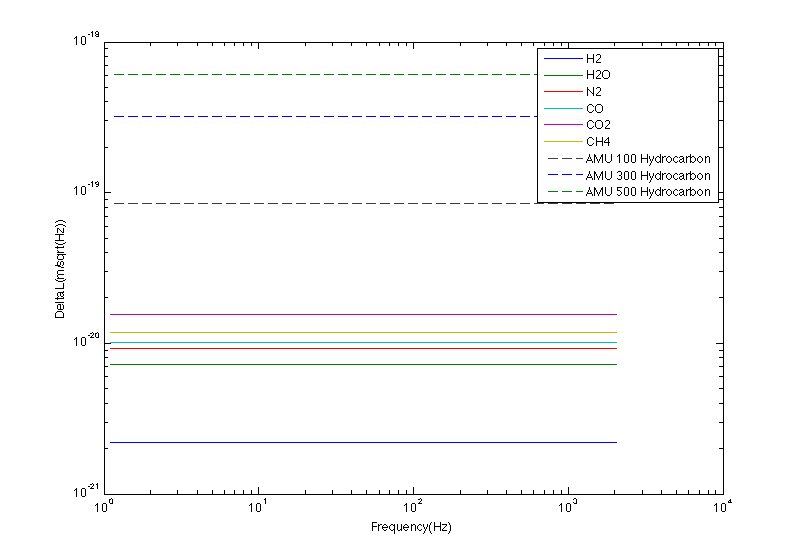
\includegraphics[width=15cm]{./figures/trapgasnoise_1.png}
	\caption[Gas Noise Comparison]{Gas Noise for 1e-6 Torr}
	\label{fig:gas_noise1}
\end{figure}

If we have a residual gas analyzer that detects a minimum partial pressure of 5e-11 Torr:

\begin{figure}[htbp]
	\centering
		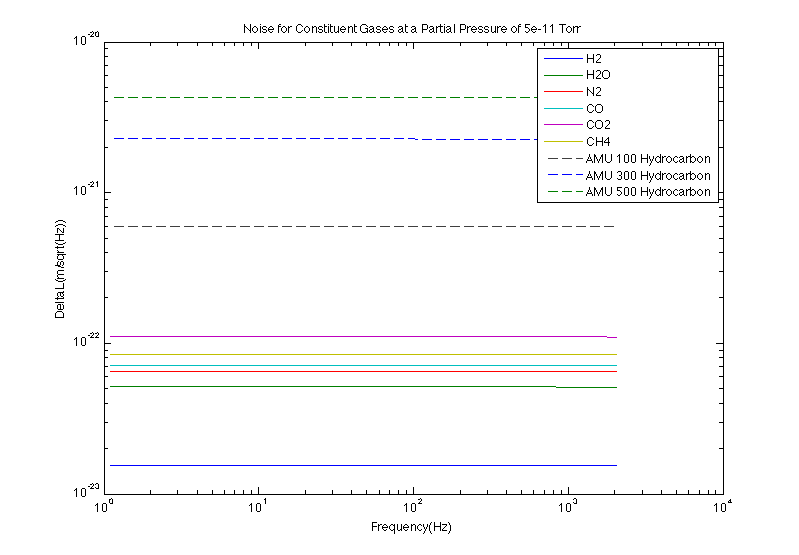
\includegraphics[width=15cm]{./figures/trapgasnoise_2.png}
	\caption[Gas Noise Comparison]{Gas Noise for 5e-11 Torr}
	\label{fig:gas_noise2}
\end{figure}

%\section{Epoxy Thermal Noise}
%
%Brownian thermal noise estimates for epoxy joints are gotten from basic application of the fluctuation-dissipation theorem. The form that we start with is,
%\begin{align*}
%S_{x^2}(f) = \frac{4 k_B T}{\omega^2} \Re(Z^{-1}), 
%\end{align*}
%where $Z$ is the impedance, $F / v$. The force equation that we use is of the form,
%\begin{align*}
%F_{\mathrm{ext}} = m \ddot{x} + k x,
%\text{where k is a complex number}, (1 + i \phi)
%\end{align*}
%
%\section{Derivation}
%
%\begin{align*}
%d_n = d(t-\tau_n)
%\end{align*} \\
%
%\begin{align*}
%d_n = d \left( t - \frac{(2n -1)}{c} L_0 - d_1 - \sum_{l=2}^{n} 2 d_l \right)
%\end{align*} \\

